\documentclass[tikz]{standalone}
\usepackage{tikz}
\usepackage{amssymb}
\usetikzlibrary{positioning}
\usetikzlibrary{calc}
\usetikzlibrary{arrows,shapes,snakes,automata,petri}
\begin{document}
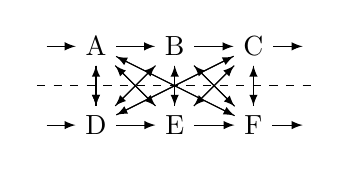
\begin{tikzpicture}
\node[](startA) at (-0.75,0){};
\node[](startD) at (-0.75,-1){};
\node[](A) at (0,0){A};
\node[](B) at (1,0){B};
\node[](C) at (2,0.0){C};
\node[](D) at (0,-1){D};
\node[](E) at (1,-1){E};
\node[](F) at (2,-1){F};
\node[](endC) at (2.75,0){};
\node[](endF) at (2.75,-1){};

\draw[dashed](-0.75,-0.5)--(2.75,-0.5);

\path
(startA) edge[-latex]node{} (A)
(startD) edge[-latex]node{} (D)
(A) edge[-latex]node{} (B)
(B) edge[-latex]node{} (C)
(D) edge[-latex]node{} (E)
(E) edge[-latex]node{} (F)
(A) edge[-latex]node{} (D)
(A) edge[-latex]node{} (E)
(A) edge[-latex]node{} (F)
(A) edge[-latex]node{} (D)
(B) edge[-latex]node{} (E)
(B) edge[-latex]node{} (F)
(B) edge[-latex]node{} (D)
(C) edge[-latex]node{} (E)
(C) edge[-latex]node{} (F)
(C) edge[-latex]node{} (D)
(D) edge[-latex]node{} (A)
(D) edge[-latex]node{} (B)
(D) edge[-latex]node{} (C)
(E) edge[-latex]node{} (A)
(E) edge[-latex]node{} (B)
(E) edge[-latex]node{} (C)
(F) edge[-latex]node{} (A)
(F) edge[-latex]node{} (B)
(F) edge[-latex]node{} (C)
(C) edge[-latex]node{} (endC)
(F) edge[-latex]node{} (endF);
\end{tikzpicture}
\end{document}